\chapter{Aquisição e Tratamento dos Dados}	

\section{Aquisição de Dados}

No âmbito do projeto SUBSAL, realizado conjuntamente entre o Observatório Nacional e a Petrobras,  instalou-se 24 estações sismográficas temporárias banda larga (STS2 ou Reftek RT151-120s). Cuja a faixa de frequência registrada varia de 50 Hz até 100 segundos. Acoplado a este sistema temos um conjunto de baterias, reguladores, painel solar e o registrador, onde são armazenados os dados. O sistema armazena os dados em um disco de 4Gb que é retirado nas campanhas de coleta.

Mesmo se tratando de estações temporárias, as instalações devem conter os requisitos mínimos para a uma aquisição confiável dos dados. Principalmente assegurar que o sensor e o registrador não sofram com as intempéries climáticas ou com danos causados pela passagem de animais ou pessoas pelo local. A Figura \ref{instalacao} mostra como é o fluxo de trabalho dos funcionários do Observatório Nacional no campo para a instalação das estações sismográficas temporárias. 

A Figura \ref{instalacao}-A mostra que o sensor deve ser acoplado à rocha sã. Com a ajuda de uma bússola o sensor é orientado segundo um azimute.  Porém para um isolamento térmico, crucial para o bom funcionamento do sismômetro, pinta-se a área com um tinta isolante e o sismômetro é revestido com uma manta térmica, como pode ser visto na A Figura \ref{instalacao}-B e C. Logo após instala-se as baterias e o sensor é mais uma vez revestido. Para a absorçao da umidade de todo o sistema da estaçao, utiliza-se carvão e sílica em gel, como pode ser visto na Figura \ref{instalacao}-D. Em seguida todo o sistema é coberto por uma nova estrutura para evitar as intempéries e cercada para isolar a área, como pode ser visto nas Figuras \ref{instalacao}-E e F.	  

\begin{figure}[!ht]
\centering
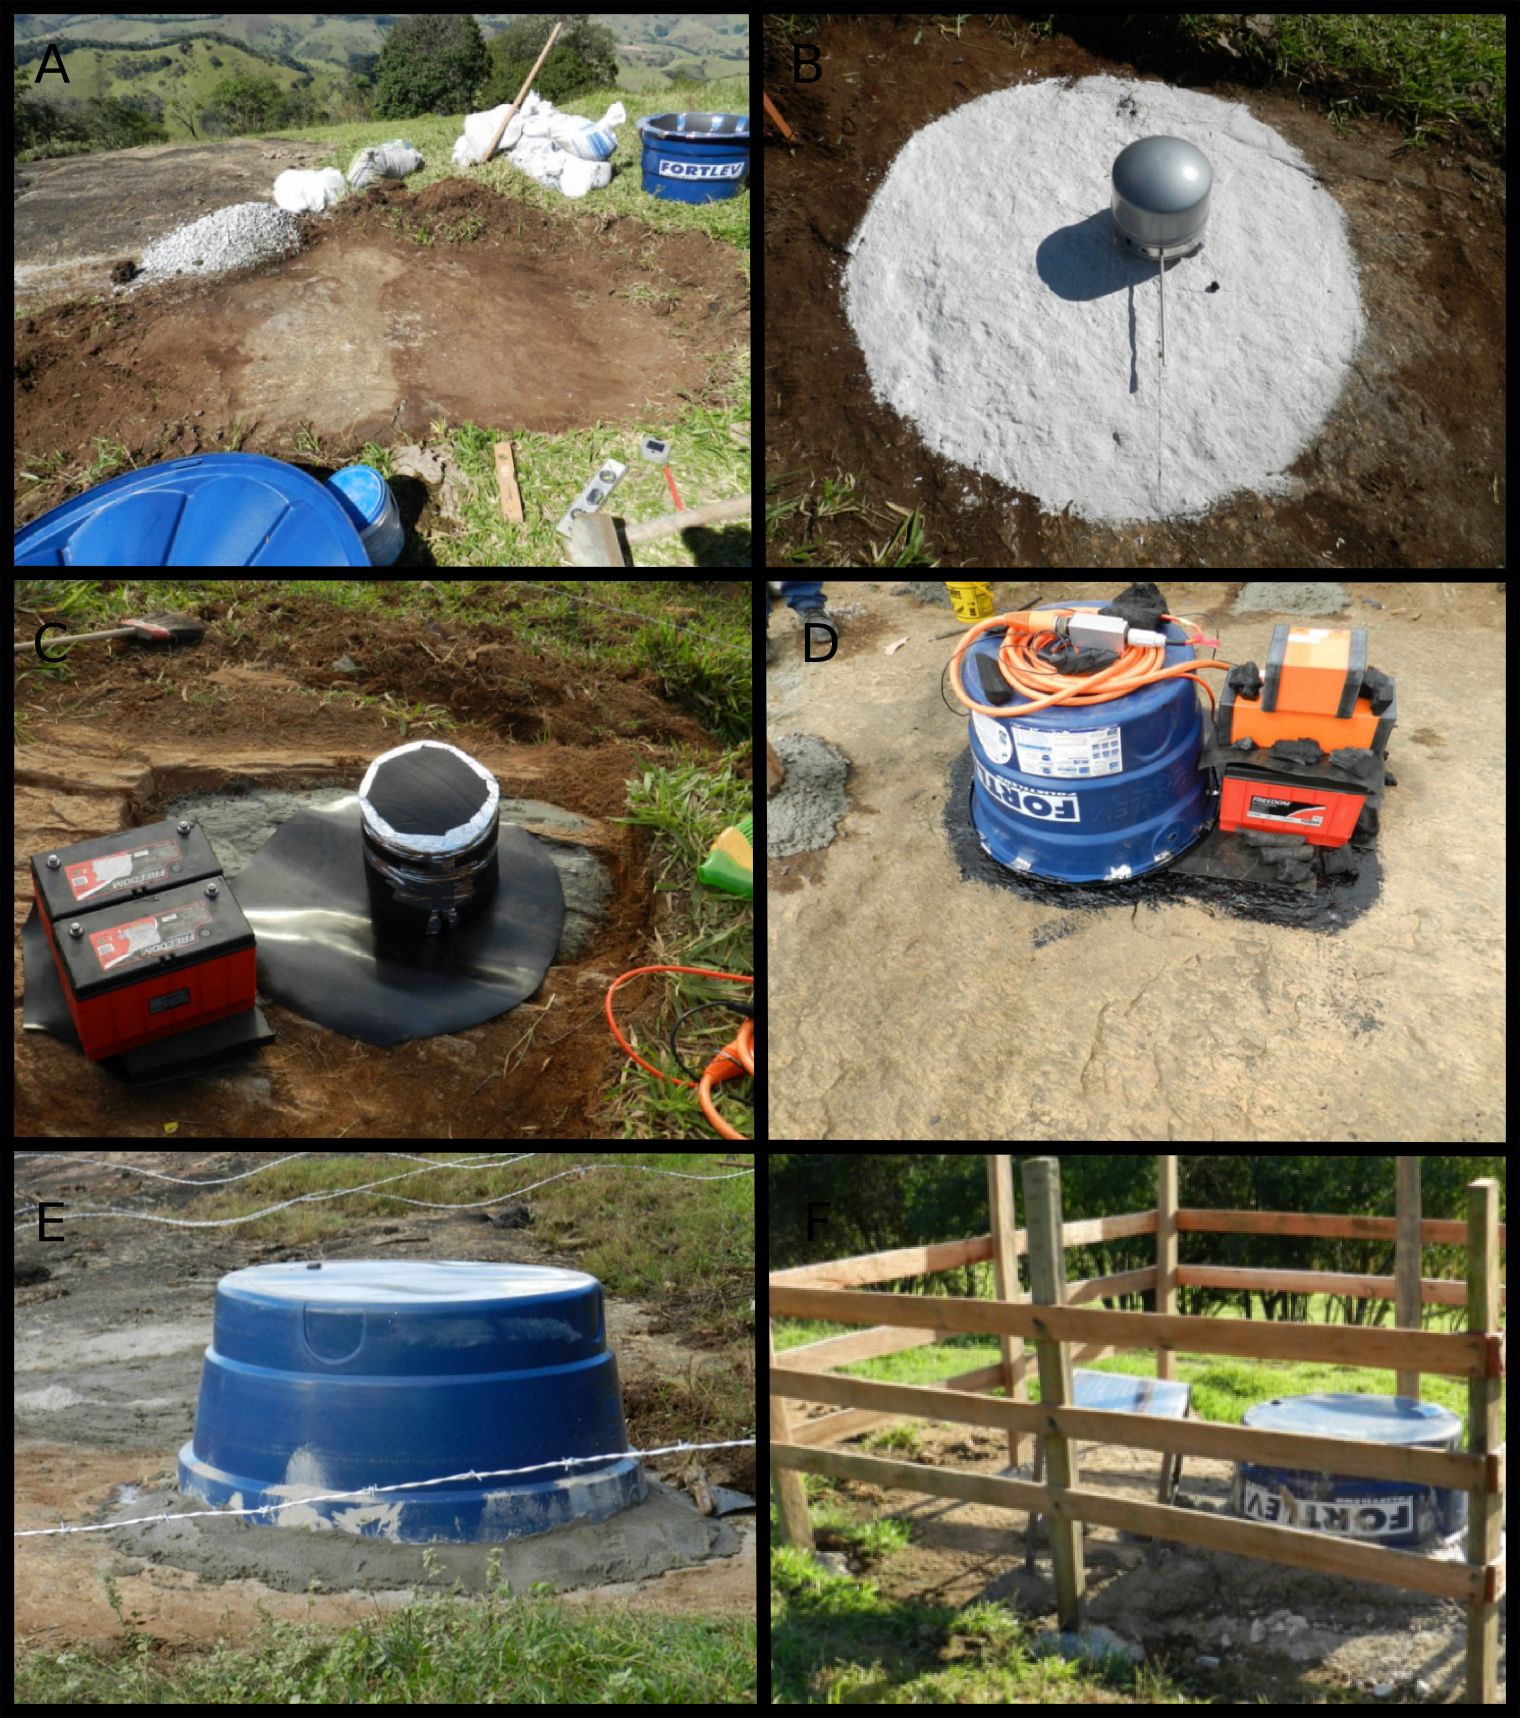
\includegraphics[scale=0.5]{instalacao.png}
\caption{Mosaico mostrando como é feita a instalação das estações sismográficas temporárias do projeto SUBSAL. As figuras mostram os diferentes estágios na instalação das estações.}
\label{instalacao}
\end{figure} 

As estações foram dispostas espacialmente em trẽs perfis em relação à costa, dois perpendiculares à costa, perfil 1 a oeste e perfil 2 a leste, e um paralelo, perfil 3, como observado na Figura \ref{map_loc}. O perfil 1 estende-se da estação STA01, localizada próximo à costa, até a STA09. O perfil 2 vai da estação STA10, ao norte, até a STA16, próximo à costa. O perfil 3 é da estação STA17, oeste, até a STA24, leste. A distância entre as estações é aproximativamente de 20 km. As coordenadas das estações são dadas na Tabela \ref{tabela1}. 

\begin{figure}[!ht]
\centering
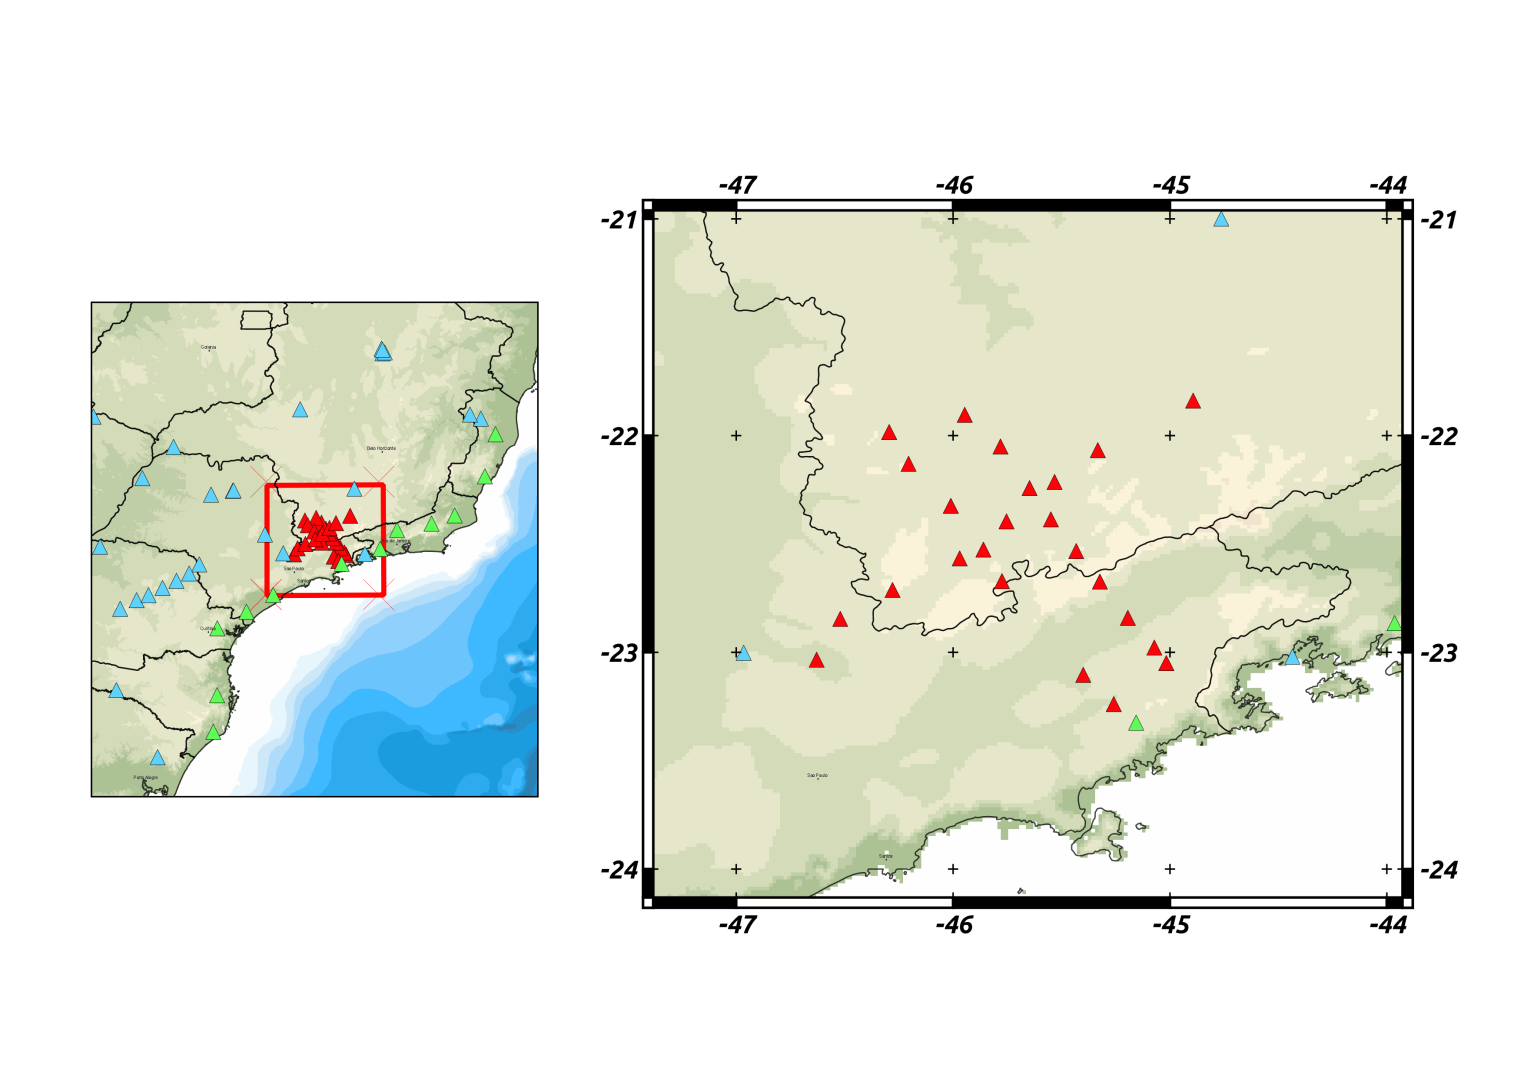
\includegraphics[scale=0.4]{mapa_das_estacoes_simosgraficas_instaladas.png}
\caption{Mapa das estações sismográficas instaladas (triângulos vermelhos). Os outros triângulos são estações da Rede Sismográfica Brasileira.}
\label{map_loc}
\end{figure}

O período de operação das estações foi distinto para os perfis. Os dois perfis perpendiculares à costa foram instalados no meio do ano de 2012 e o perfil paralelo no final de 2012. As estações ficaram em fucionamento até o final do ano de 2013 registrando o movimento do terreno de maneira contínua. 

O produto do deslocamento das partículas do meio registrado pelo sismógrafo, através de sensores verticais e horizontais em três componentes, pode ser visto na Figura \ref{simograma}. Esse registro da variação da amplitude em uma série temporal é chamado de sismograma. 

\begin{figure}[!ht]
\centering
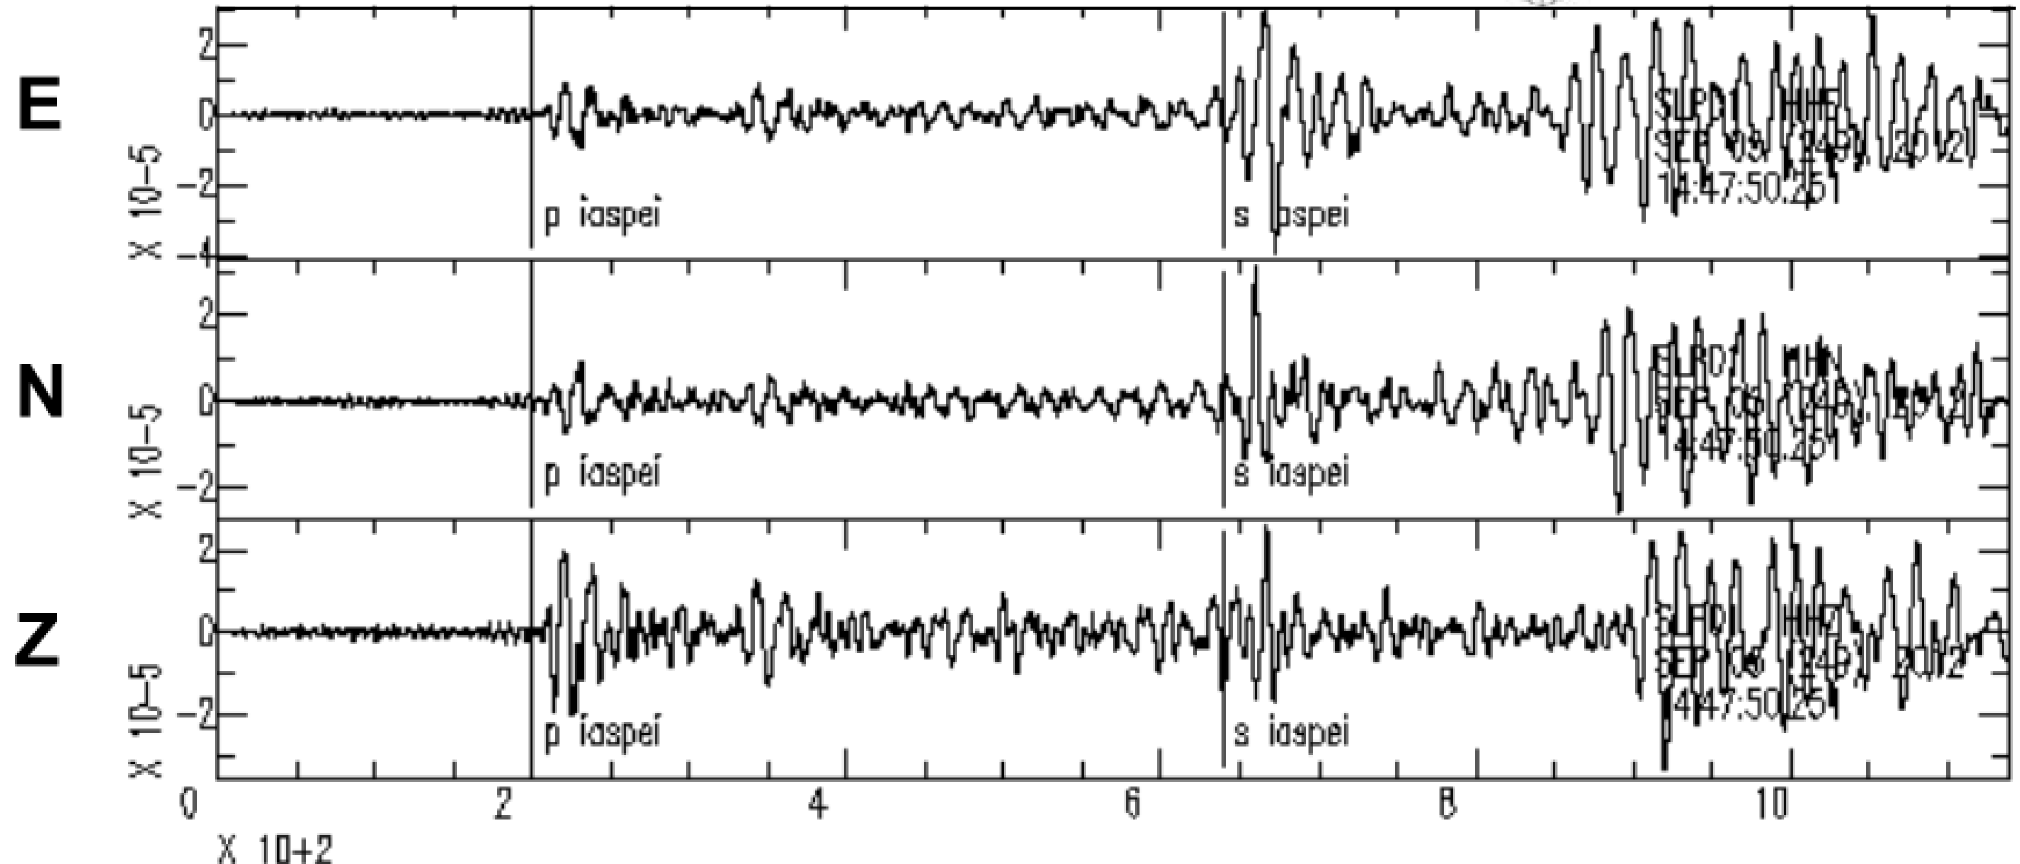
\includegraphics[scale=0.6]{sismograma.png}
\caption{Sismograma mostrandos as três componentes do deslocamento do terreno.}
\label{simograma}
\end{figure}

O sismograma é gerado pela perturbação do meio pelas ondas  mecânicas que se propagam no interior da Terra. Essas ondas  tem velocidades variando em função dos parâmetros elásticos do meio e da densidade. E estes variam pela mineralogia e condições de pressão e temperatura do meio atravessado. As ondas mecânicas são divididas em ondas de corpo e de superfície. As ondas de corpo estão categorizadas em dois tipos: as ondas P, longitudinal, e as ondas S, transversais. A onda P é mais rapida e que consegue se propagar em todos os meios, tem velocidade entre 4 e 7 km$/$s na crosta terrestre e em torno de 8 km$/$s no manto superior. As ondas S tem velocidade menor do que a onda P, em torno de 3 a 4 km$/$s na crosta.

Para produzir esta análise sobre a estrutura da região de estudo utilizou-se de um conjunto de dados com eventos sísmicos registrados. O número de eventos utilizados no processamento varia devido ao nível de sinal-ruído da forma da onda, pois há uma necessidade de visualização clara da chegada da onda P, como pode ser constatado na Figura \ref{simograma} .

\section{Tratamento dos Dados}

A caracterização prévia das informações contidas no sinal é imprescindível para o processamento. A avaliação da performance e da qualidade dos dados da estações sismográficas foram feitas no software livre PQLX.  A metodologia do PQLX é baseada no trabalho de \cite{McNamara_Buland_2004}. Esse procedimento é bastante usado para se obter a informação espectral sísmica.

No programa PQLX a série temporal é segmentada em intervalos de uma hora, com 50\% de superposição do sinal. Cada janela de hora está separada em 13 intervalos com 75\% de superposição para calcular a “Power Spectral Density”. As médias obtidas para cada um dos 13 intervalos são usadas para estimar a “Probability Density Functions”, calculados a partir das médias pelo número total de segmentos de hora em hora. 

Essa metodologia de \cite{McNamara_Buland_2004} difere dos métodos habitualmente utilizados, porque não é necessário a visualização de todo conjunto de dados para uma estima qualitativa do sinal, observado na Figura \ref{PQLX}.

\begin{figure}[!ht]
\centering
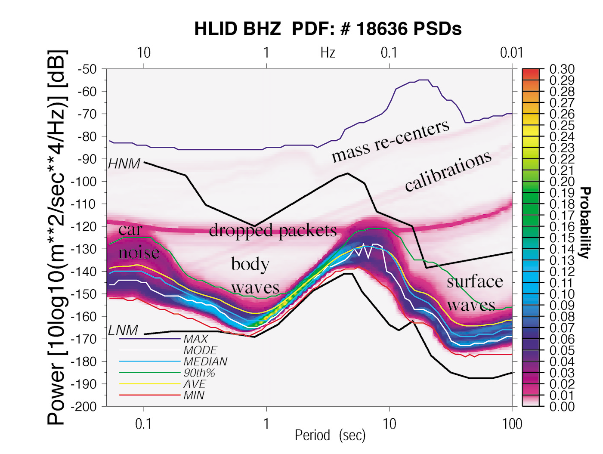
\includegraphics[scale=0.6]{mcnamura_buland.png}
\caption{Análise qualitativa do sinal atraves das \textit{Power Density Functions}. \cite{McNamara_Buland_2004} }
\label{PQLX}
\end{figure}

O produto de uma análise qualitativa premilinar nos gráficos gerados pelo programa PQLX é mostrado na Figura \ref{PQLX_results}, que tem como exemplos a componente HHZ nas estações STA05, STA04 e STA24. Observando os resultados nas estações temporárias conclui-se que existem registros bons e confiáveis, como exemplo a Figura \ref{PQLX_results}-A. Porém em algumas estações existem pequenos problemas, que são caracterizados por tendências lineares, como observados na Figura \ref{PQLX_results}-B. Já em outras estações pode-se constatar neste estudo preliminar a falta de registros na componente HHZ, que possivelmente é um problema no instrumento registrador ou no sensor, isto pode ser observado na Figura \ref{PQLX_results}-C.

\begin{figure}[!ht]
\centering
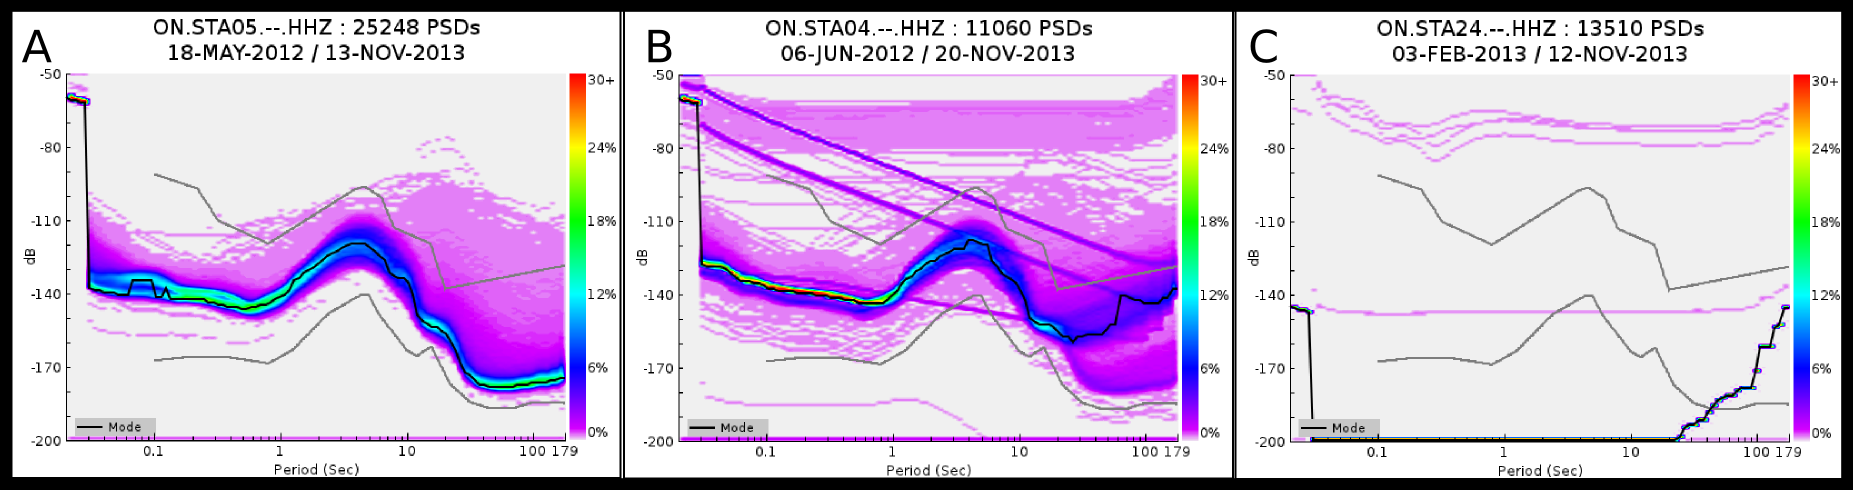
\includegraphics[scale=0.35]{pqlx_results.png}
\caption{Exemplos de resultados gerados pela análise qualitativa do sinal atraves do programa PQLX, que utiliza o método de \cite{McNamara_Buland_2004}.}
\label{PQLX_results}
\end{figure}

\subsection{Função do Receptor}

Os dados utilizados para os cálculos utilizando o método da Função do Receptor foram dados coletados das 24 estações temporárias da Rede SUBSAL e a estação permanente SLP01, esta pertecente a rede RSIS. Po, como pode ser visto na Figura \ref{map_loc}. Porém ao final agregou-se valores da profundidade de Moho de estações pertencentes à USP. 

Para assegurar a confiabilidade do processamento é necessário um tratamento preliminar dos sinais brutos. Utilizou-se eventos catalogados na rede IRIS para uma identificação automática nestes sinais. Alguns pré-requisitos foram utilizados para a escolha dos eventos, como:

\begin{enumerate}
\item Distância Epicentral;
\item Magnitude;
\end{enumerate}

Sismos próximos, com distância menor que 20 graus da estação estudada, geram ondas com incidência oblíqua e esse tipo de dado deve ser utilizado com cuidado. Em sismos com distâncias maiores que 95 graus as ondas P não chegam na estação devido a inversão de velocidade no limite manto-núcleo, diminuição da velocidade da onda P entre o manto e o núcleo, e não é observada a onda P direta. Por isso a distância epicentral é tida como ideal entre 20 e 95 graus, como é observado na Figura \ref{mapa_eventos}. Devido grande parte dos sismos serem oriundos da Cordilheira dos Andes,como é visto na Figura \ref{teste_tempo}, também utilizou-se dados comn distância menor que 20 graus. A magnitude do sismo é importante para a propagação da onda, eventos com pequena magnitude não tem energia suficiente para gerar energia suficiente para gerar um sinal claro no sismograma.

\begin{figure}[!ht]
\centering
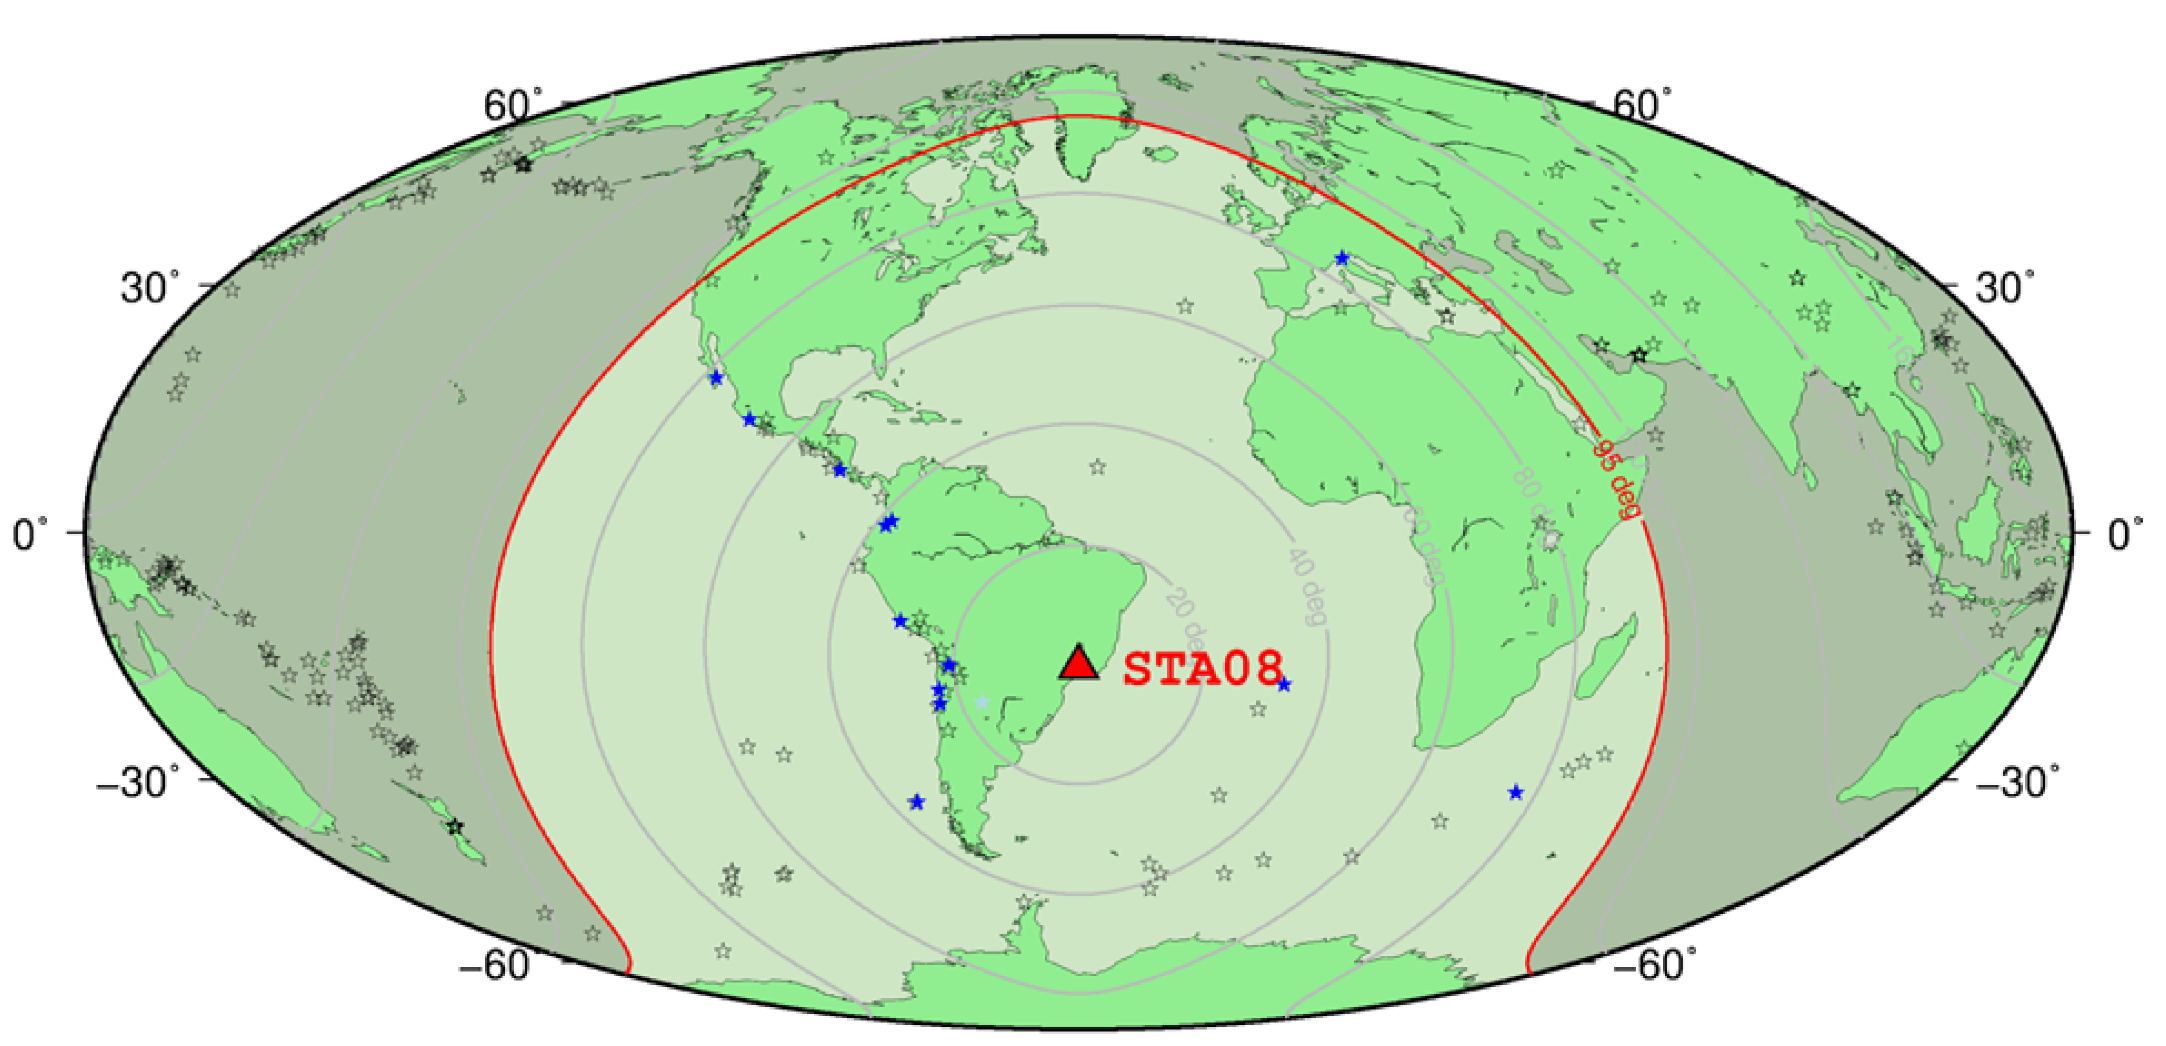
\includegraphics[scale=0.6]{mapa_de_eventos.png}
\caption{Mapa dos eventos (estrelas) registrados na estação STA08. O limite de 95 graus está indicada em vermelho. Estrelas azuls mostram os eventos com dados de qualidade que são usadas no calculo das Funçoes do Receptor}
\label{mapa_eventos}
\end{figure}

Subsequentemente um janelamento do registro em 5 segundos antes e 10 segundos depois da chegada da onda P, esta é calculada pelo modelo de velocidade da Terra  IASPEI91 \citep{kennet_iaspei_1991}. Após a discriminação e o janelamento do sinal, examina-se visualmente cada registro para certificar que todos os eventos selecionados tem um nível de sinal-ruído bom, como na Figura \ref{simograma} . 

Logo após removeu-se a média e tendência linear dos dados. Aplicou-se um filtro passa-alta com freqüência de corte de 0.1 Hz para eventos com distância entre 20 e 95 graus e de 2 Hz para eventos próximos (<20). Os dados originais com amostragens a cada 0,01 segundos (100 Hz) são interpolados para gerar dados com amostragens cada 0,025 segundas (40 Hz), porque a informação de alta freqüência não é considerada nesta análise.

Após esta análise preliminar nos dados observou-se que algumas estações temporárias apresentaram problemas nos dados e tiveram que ser descartadas dessa análise. Tais estações foram: STA22, STA23 e STA24.


\subsection{Dispersão de Ondas de Superfície}

Para o cálculo da dispersão das ondas de superfície utilizou-se além das estações temporárias da Rede SUBSAL as estações da Rede RSIS que estão próximas à área de estudo.

A garantia da fiabilidade do tempo de chegada da onda P é fundamental para o processamento gerar resultados consistentes. Portanto testes com o tempo de chegada da onda P forão feitos. \cite{gibbons_identification_2006} mostra que fazen do a correlação de dois eventos distantes em uma estação sismográfica consegue-se caracterizar esse tempo de chegada, como é visto na Figura \ref{teste_tempo}. \cite{gibbons_identification_2006} assume que  se não há alterações mensuráveis na velocidade da estrutura entre a fonte e os receptores, ondas sísmicas de dois eventos co-localizados terá a mesma duração de tempo para chegar a um determinado sensor. A função de correlação cruzada para um dado sinal a uma dada estação mede que a semelhança entre a porção posterior do sismograma é a do modelo de forma de onda. O tempo de separação entre o início do modelo e o valor máximo da função de correlação cruzada deve ser igual ao tempo que separa os dois tempos de origem dos eventos para todas as estações. Qualquer discrepância nos tempos de separação medido em duas estações diferentes, o que não é atribuível a diferença entre fontes ou uma SNR baixa, deve ser o resultado de uma anomalia em sincronismo um, ou ambos, dos instrumentos.

\begin{figure}[!ht]
\centering
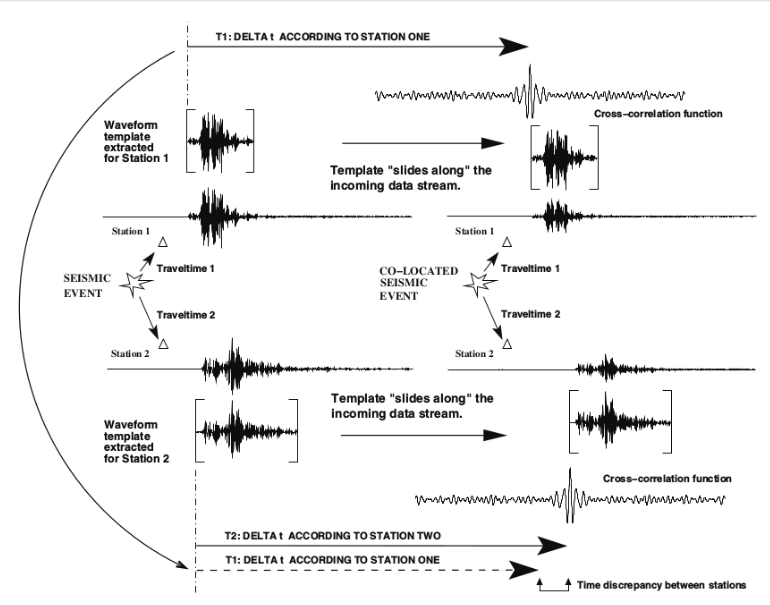
\includegraphics[scale=0.7]{correlacao_tempo_de_chegada.png}
\caption{Uma ilustração esquemática de como dois eventos sucessivos de fontes sísmicas quase idênticas que podem ser explorados para revelar anomalias dos tempo de chegada da onda P numa dada estação. \citep{gibbons_identification_2006}}
\label{teste_tempo}
\end{figure}

Nesste trabalho utilizamos uma metodologia semelhante a de \cite{gibbons_identification_2006}. Utilizou-se um sismo distante de um par de estações sismográficas próximas. Com os sinais registrados fez-se a correlação cruzada dos dados. Como a fonte está distante das estações a correlação dos sinais deve ser próxima de zero. Este teste do tempo de chegada da onda P é para garantir a confiabilidade dos dados das estações temporárias. Portanto em cada par de estações correlacionadas sempre tinha uma estação permanente, estação com dados confiáveis.

\begin{figure}[!ht]
\centering
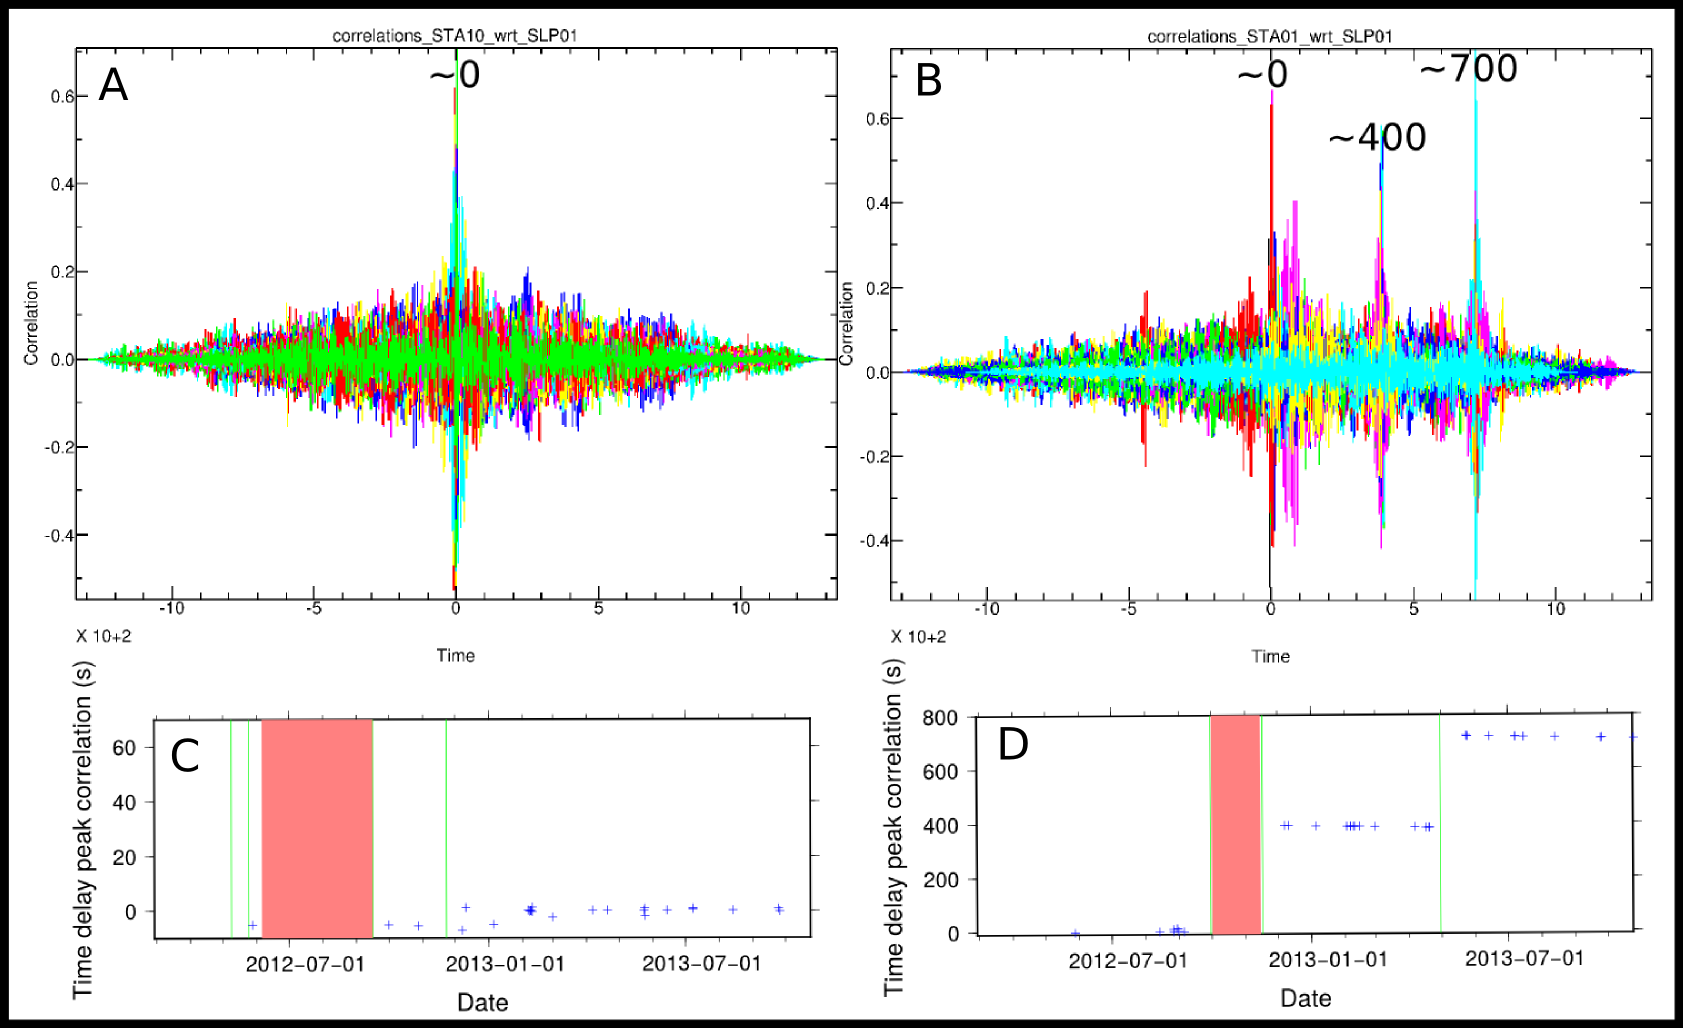
\includegraphics[scale=0.4]{correlacao_tempo_de_chegada_resultado.png}
\caption{Correlação de eventos sucessivos de fontes sísmicas entre duas estações sismográficas (A e B). Na parte inferior mostram o atraso do tempo de chegada da onda P da correlação pelo tempo. As retas verticais mostram os períodos onde teve manutenção do equipamento (C e D).}
\label{teste_tempo_results}
\end{figure}

Os gráficos gerados com a correlação são vistos na Figura \ref{teste_tempo_results}. Os resultados mostram que para algumas estações temporárias há erros na chegada da onda P, como visto na Figura \ref{teste_tempo_results}-B. Tais erros podem ter sidos gerados por difentes fatores, como erro no sinal do GPS acoplado à estação, erro instrumental ou até mesmo erro no momento da manutenção da estação. Na Figura \ref{teste_tempo_results}-C e D encontramos um gráfico mostrando o tempo de atraso das correlações pelo tempo. As linhas verticais(verdes) nos gráficos mostram intervalos onde foram feitas manutenções nas estações temporárias. Vemos que na Figura \ref{teste_tempo_results}-D, que após as manutenções na estação STA01, erros sistemáticos apareceram nos registro e isso pode ser confirmado na Figura \ref{teste_tempo_results}-B.

Com esse tratamento preliminar dos dados pôde-se selecionar melhor o banco de dados e tentar minimizar os erros gerados no processamento da dispersão das curvas de superfície. Após estes estudos, as estações temporárias STA22, STA23, e STA23 foram consideradas impróprias para o cálculos da dispersão das ondas Rayleigh. Porém serão aproveitadas quando for analisada a dispersão das ondas Love. 
